% !TEX root=../../Thesis.tex
\chapter{Accounting for the uncertainty}\label{ch:uncertainty}
% \begin{center}
% 	\textit{\textbf{RQ 2: In what way can an \gls{rl} agent utilize the uncertainty of its predictions and actions?}}
% 	% \textit{\textbf{RQ 4: How can the quality of a RL agent be improved by accounting for uncertainty?}}
% 	\end{center}
% 	\vspace{12pt}

The motivation of handling uncertainty. In this chapter we present two approches to handling the uncertainty, one is the uncertainty in output of the \gls{dqn} and the other in the uncertainty of the intention estimation that is feed as an input to the \gls{dqn}.


\section{Uncertainty of the decision}
\tommy{NN is a black box. The utility value q that come from the DQN works great if it was trained on the }


\subsection{Approach}
One limitation of the DQN algorithm is that only the maximum likelihood estimate of the $Q$-values is returned. The risk of taking a particular action can be approximated as the variance in the estimated $Q$-value~\cite{Garcia2015}. One approach to obtain a variance estimation is through statistical bootstrapping~\cite{Efron1982}, which has been applied to the DQN algorithm~\cite{Osband2016}. The basic idea is to train an ensemble of neural network on different subsets of the available replay memory. The ensemble will then provide a distribution of $Q$-values, which can be used to estimate the variance. Osband et al. extended the ensemble method by adding a randomized prior function (RPF) to each ensemble member, which gives a better Bayesian posterior~\cite{Osband2018}. The $Q$-values of each ensemble member $k$ is then calculated as the sum of two neural networks, $f$ and $p$, with equal architecture, i.e.,
%
\begin{align}
	Q_k(s,a) = f(s,a;\theta_k) + \beta p(s,a;\hat{\theta}_k).
\end{align}
%
Here, the weights $\theta_k$ of network $f$ are trainable, and the weights $\hat{\theta}_k$ of the prior network $p$ are fixed to the randomly initialized values. A parameter $\beta$ scales the importance of the networks. With the two networks, the loss function in Eq.~\ref{eq:loss} becomes
%
\begin{align}
	\label{eq:loss_boot}
	L(\theta_k) = \mathbb{E}_M \Big[ & (r + \gamma \max_{a'} (f_{\theta^-_k}+\beta p_{\hat{\theta}_k})(s',a') \nonumber \\
	& - (f_{\theta_k}+ \beta p_{\hat{\theta}_k})(s,a) )^2 \Big].
\end{align} 

Algorithm~\ref{alg:training} outlines the complete ensemble RPF method, which was used in this work. An ensemble of $K$ trainable and prior neural networks are first initialized randomly. Each ensemble member is also assigned a separate experience replay memory buffer $m_k$ (although in a practical implementation, the replay memory can be designed in such a way that it uses negligible more memory than a shared buffer). For each new training episode, a uniformly sampled ensemble member, $\nu \sim \mathcal{U}\{1,K\}$, is used to greedily select the action with the highest $Q$-value. This procedure handles the exploration vs. exploitation trade-off and corresponds to a form of approximate Thompson sampling. Each new experience $e = (s_i, a_i, r_i, s_{i+1})$ is then added to the separate replay buffers $m_k$ with probability $p_\mathrm{add}$. Finally, the trainable weights of each ensemble member are updated by uniformly sample a mini-batch $M$ of experiences and using stochastic gradient descent (SGD) to backpropagate the loss of Eq.~\ref{eq:loss_boot}.

\begin{algorithm}[h]
	\caption{Ensemble RPF training process}\label{alg:training}
	\begin{algorithmic}[1]
		\For{$k \gets 1$ to $K$}
			\State Initialize $\theta_k$ and $\hat{\theta}_k$ randomly
			\State $m_k \gets \{\}$
		\EndFor
		\State $i \gets 0$
		\While{networks not converged}
			\State $s_i \gets $ initial random state
			\State $\nu \sim \mathcal{U}\{1,K\}$%, where $k \in \mathbb{N}$
			\While{episode not finished}
				\State $a_i \gets \argmax_{a} Q_\nu(s_i,a)$
				\State $s_{i+1}, r_i \gets $ \Call{StepEnvironment}{$s_i, a_i$}
				% \For{$i \in \{1,\dotsc,K\}$}
				\For{$k \gets 1$ to $K$}
					\If{$p \sim \mathcal{U}(0,1) < p_\mathrm{add}$}%, where $p \in \mathbb{R}$ 
						\State $m_k \gets m_k \cup \{(s_i, a_i, r_i, s_{i+1})\}$
					\EndIf
					\State $M \gets $ sample mini-batch from $m_k$
					\State update $\theta_k$ with SGD and loss $L(\theta_k)$
				\EndFor
				\State $i \gets i + 1$
			\EndWhile
		\EndWhile
	\end{algorithmic}
\end{algorithm}

\begin{align*}
r_t = &\begin{cases}
1 & \text{at reaching the goal, }\\
-1 & \text{at a collision},\\
-\left(\frac{j_t}{j_{\max}}\right)^2\frac{\Delta \tau}{\tau_\mathrm{max}} & \text{at non-terminating steps.}
% \label{eq:reward}
\end{cases} 
\end{align*}


\tommy{Confidence criterion}

The agent's uncertainty in choosing different actions can be defined as the coefficient of variation\footnote{Ratio of the standard deviation to the mean.} $c_\mathrm{v}(s,a)$ of the $Q$-values of the ensemble members.  
In previous work, we introduced a confidence criterion that disqualifies actions with $c_\mathrm{v}(s,a) > c_\mathrm{v}^\mathrm{safe}$, where $c_\mathrm{safe}$ is a hard threshold~\cite{Hoel2020}. 
The value of the threshold should be set so that $(s,a)$ combinations that are contained in the training distribution are accepted, and those which are not will be rejected. This value can be determined by observing values of $c_\mathrm{v}$ in testing episodes within the training distribution, see Sect.~\ref{sec:resultsWithinDistribution} for further details. 


% A high uncertainty, where $c_\mathrm{v}(s,a) > c_\mathrm{v}^\mathrm{safe}$, indicates that $(s,a)$ is outside the training distribution. The parameter value $c_\mathrm{safe}$ can be set just above the observed values of $c_\mathrm{v}$ in testing episodes within the training distribution, see Sect.~\ref{sec:resultsWithinDistribution} for further details.

When the agent is fully trained (i.e., not during the training phase), the policy chooses actions by maximizing the mean of the $Q$-values of the ensemble members, with the restriction $c_\mathrm{v}(s,a) < c_\mathrm{v}^\mathrm{safe}$, i.e.,
%
\begin{equation}
	\begin{aligned}
		\argmax_{a} \frac{1}{K} \sum_{k=1}^K Q_k(s,a),\\
		\textrm{s.t.} \quad c_\mathrm{v}(s,a) < c_\mathrm{v}^\mathrm{safe}.
	\end{aligned}
\end{equation}
%
In a situation where no possible action fulfills the confidence criterion, a fallback action $a_\mathrm{safe}$ is chosen.

\subsection{Simulated experiments}
\todo{show the difference of having the uncertainty estimate not having the estimate}

\subsection{Results and discussion}
We show two approaches of handing uncertainty. with an estimate of the uncertainty in actions we showed that it can be used to reduce collisions and risk by choosing another policy than the one trained on data it is not confident in. 

\begin{figure}[h]
	\mbox{\parbox{\textwidth}{
	\centering
	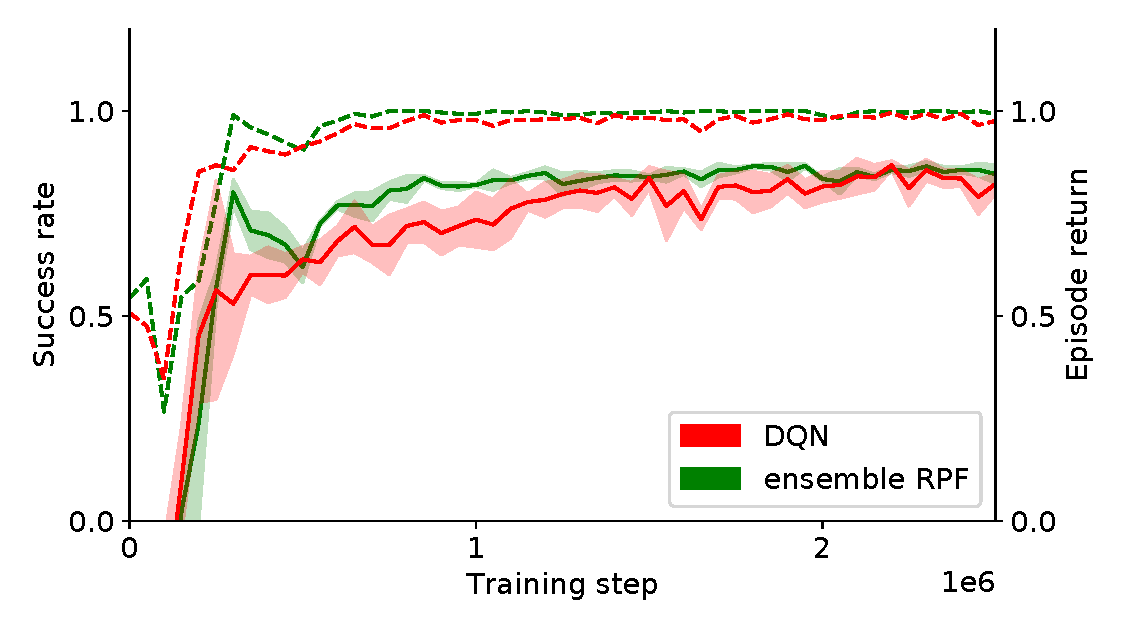
\includegraphics[width=0.99\columnwidth]{YourThesis/papers/ensamble/figures/return_success_rate_2_wo_type_3_fonts.pdf}
	}}
	\caption{Proportion of test episodes where the ego vehicle reached its goal (dashed), and episode return (solid), over training steps for the ensemble RPF and DQN methods. The shaded areas show the standard deviation for $5$ random seeds.}
	% \label{fig:returnAndSuccess}
\end{figure}

% ZZZ Change left y-axis to percent, to make it more clear that it refers to a proportion

\begin{figure}[h]
	\mbox{\parbox{\textwidth}{
	\centering
		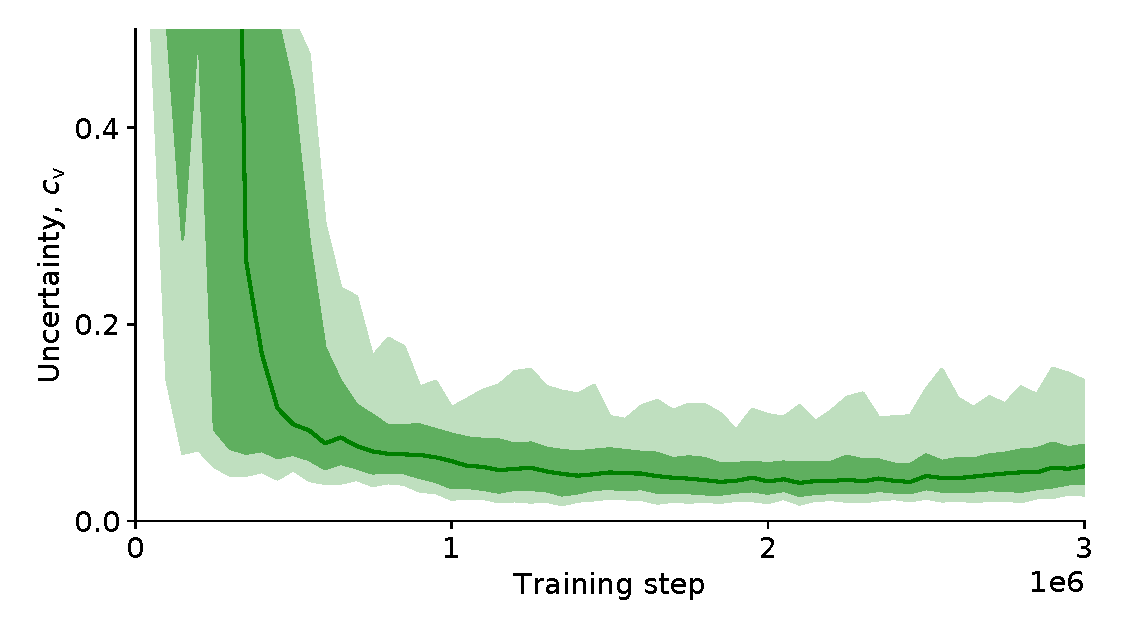
\includegraphics[width=0.99\columnwidth]{YourThesis/papers/ensamble/figures/uncertainty_3_wo_type_3_fonts.pdf}
		}}
		\caption{Mean coefficient of variation $c_\mathrm{v}$ for the chosen action during the test episodes. The dark shaded area shows percentiles $10$ to $90$, and the bright shaded area shows percentiles $1$ to $99$.}
	% \label{fig:cv}
\end{figure}

\begin{figure}[h]
	\mbox{\parbox{\textwidth}{
	\centering
		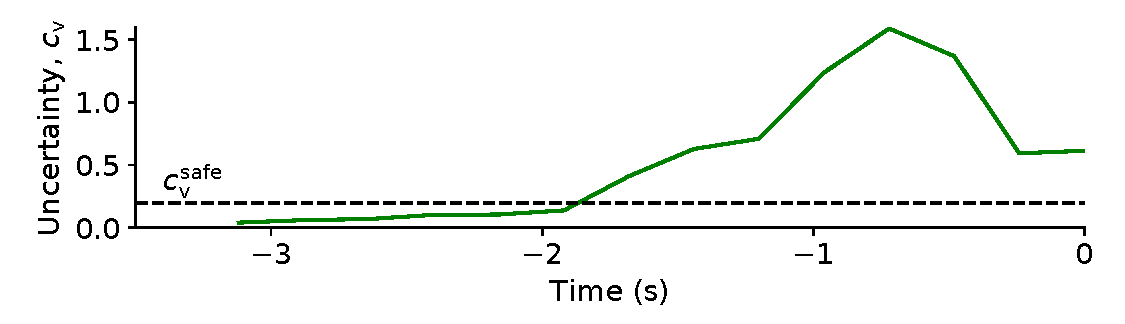
\includegraphics[width=0.99\columnwidth]{YourThesis/papers/ensamble/figures/uncertainty_at_collision_wo_type_3_fonts.pdf}
		}}
		\caption{Uncertainty $c_\mathrm{v}$ during the time steps before one of the collisions in the test episodes, within the training distribution. The collision occurs at $t=0$ s.}
	% \label{fig:cvDuringCrash}
\end{figure}

\begin{figure}[h]
	\mbox{\parbox{\textwidth}{
		\centering
	\begin{subfigure}[]{0.99\columnwidth}
	\centering
		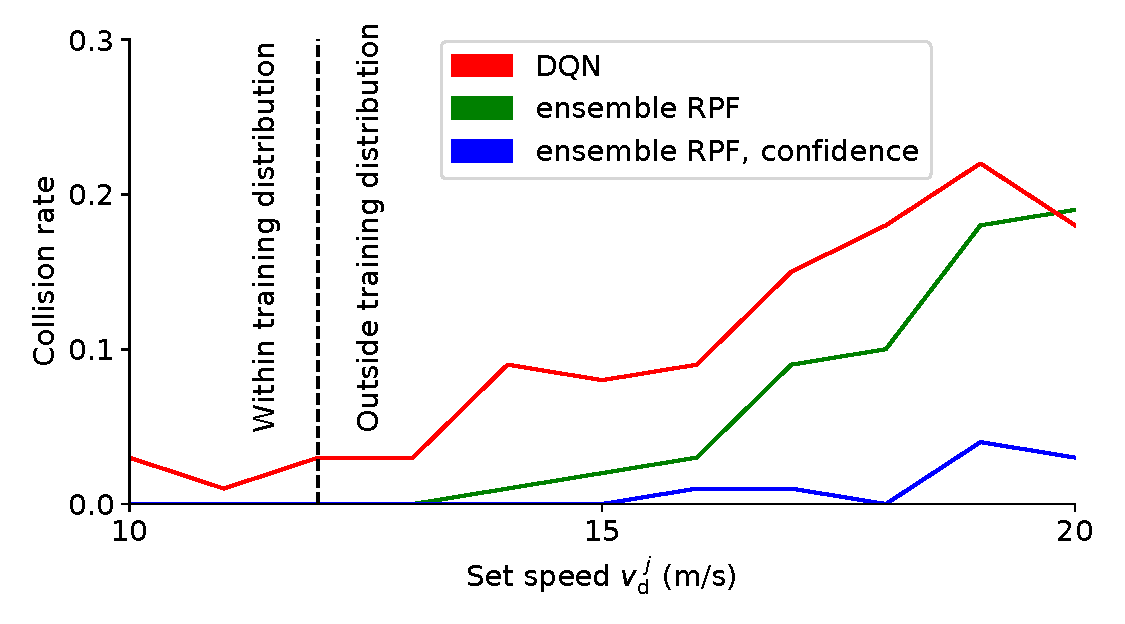
\includegraphics[width=0.99\columnwidth]{YourThesis/papers/ensamble/figures/collisions_outside_distribution_2_wo_type_3_fonts.pdf}
		\caption{Proportion of collisions.}
	\end{subfigure}
	
	\vspace{5pt}
	
	\begin{subfigure}[]{0.99\columnwidth}
	\centering
		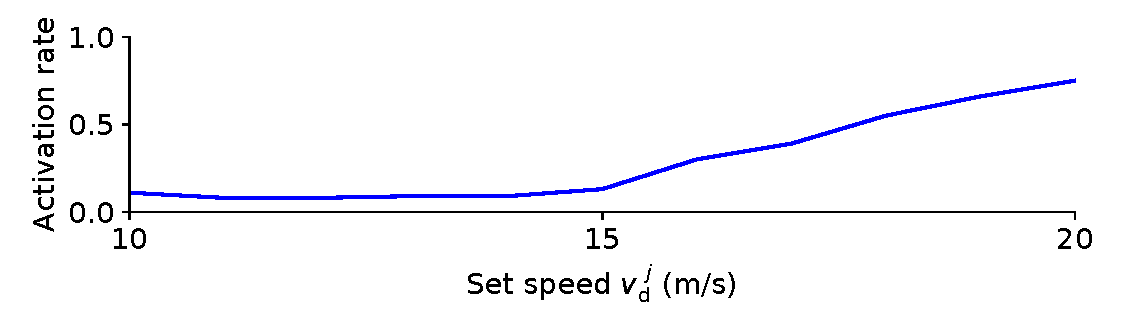
\includegraphics[width=0.99\columnwidth]{YourThesis/papers/ensamble/figures/activation_rate_2_wo_type_3_fonts.pdf}
		\caption{Proportion of episodes where $a_\mathrm{safe}$ was used at least once.}
	\end{subfigure}
	\caption{Performance of the ensemble RPF agent, with and without the confidence criterion, and the DQN agent, in test episodes with different set speeds $v_\mathrm{d}^j$ for the surrounding vehicles. %The shaded areas show the standard deviation for $5$ random seeds.
	}
	}}
	% \label{fig:performanceOutsideDistribution}
\end{figure}

% \begin{figure}[h]
% 	\mbox{\parbox{\textwidth}{
% 	\centering
% 	\begin{subfigure}[t]{0.48\columnwidth}
% 		\centering
% 		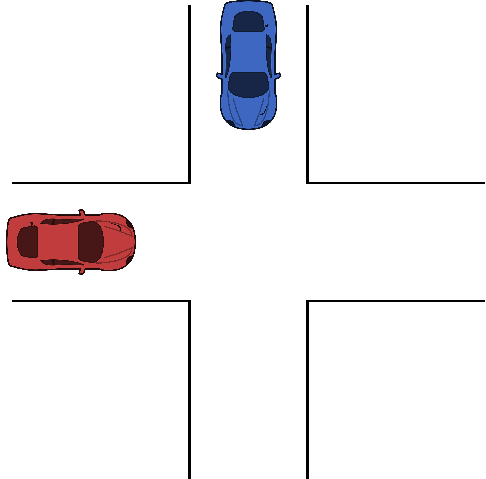
\includegraphics[width=0.7\columnwidth]{YourThesis/papers/ensamble/figures/figures-scen1.pdf}
% 		\caption{$t=0$, initial situation.}
% 	\end{subfigure}%
% 	~ 
% 	\begin{subfigure}[t]{0.48\columnwidth}
% 		\centering
% 		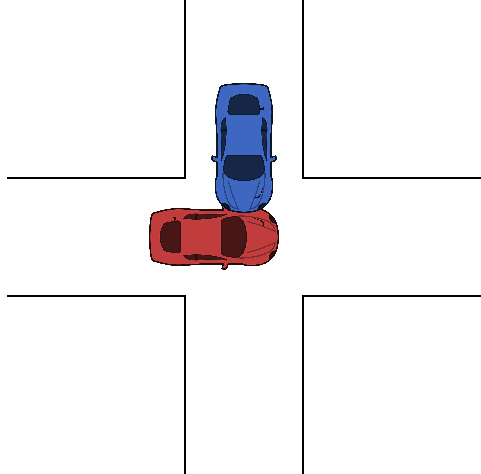
\includegraphics[width=0.7\columnwidth]{YourThesis/papers/ensamble/figures/figures-scen2.pdf}
% 		\caption{$t=1$, DQN and ensemble RPF without confidence criterion.}
% 	\end{subfigure}
	
% 	\vspace{5pt}
	
% 	\begin{subfigure}[t]{0.48\columnwidth}
% 		\centering
% 		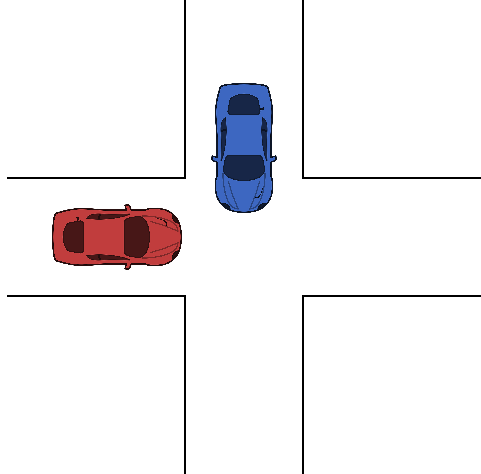
\includegraphics[width=0.7\columnwidth]{YourThesis/papers/ensamble/figures/figures-scen3.pdf}
% 		\caption{$t=1$, ensemble RPF with confidence criterion.}
% 	\end{subfigure}
% 	~ 
% 	\begin{subfigure}[t]{0.48\columnwidth}
% 		\centering
% 		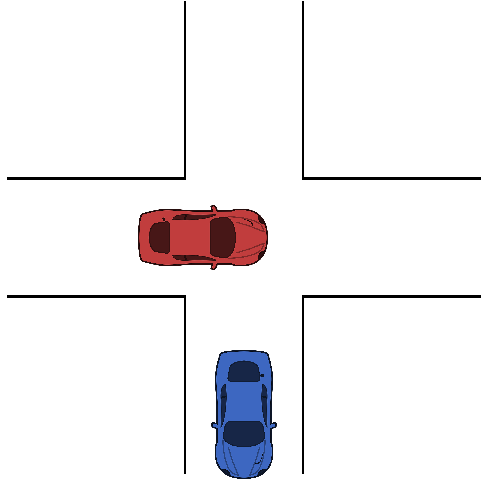
\includegraphics[width=0.7\columnwidth]{YourThesis/papers/ensamble/figures/figures-scen4.pdf}
% 		\caption{$t=1.5$, ensemble RPF with confidence criterion.}
% 	\end{subfigure}
% 	}}
% 	\caption{Example of a situation outside of the training distribution,
% 	where there would be a collision if the confidence criterion is not used. The vehicle at the top is here approaching the crossing at $20$ m/s.}
% 	% \label{fig:collisionOutsideDistribution}

% \end{figure}

We show two approaches of handing uncertainty. with an estimate of the uncertainty in actions we showed that it can be used to reduce collisions and risk by choosing another policy than the one trained on data it is not confident in. 
The other work show how bad \gls{dqn} is at handing uncertainty in the input space. The results from the experiments show that the algorithms trained with an estimate from the probability distribution outperformed the algorithm trained with the probability distribution as inputs. 

\section{Uncertainty of the intention}
In paper A the policy put itself in a position that would not be in conflict with another cars time to intersection and could avoid a lot of the collisions. But the cases the cars collided was when in somehow ended up in a collision course and thats when it had trouble making its way out. 

\subsection{Approach}


Because the state is no longer observable, the agent must reason about the history of taken actions and observations. Often, this history can be summarized in a statistic refered to as a belief, or belief state. A belief is a probability distribution over states so that $b: \mathcal{S} \rightarrow [0,1]$ and $\sum_{s} b(s)=1$, or $\int_{s} b(s)=1$ for continuous states. 

\subsection{Simulated experiments}

\subsection{Results and discussion}